\chapter{Results}
% In this chapter, you should discuss the results you have obtained from your implementation.
% These can be correctness results, i.e whether the implementation behaved as expected, or numerical results that express runtime or energy measurements.

With our polling implementation as a baseline we measured about 4.9mA, regardless of button input. As expected, the polling method consumes a lot of energy since it constantly runs instructions whether they are needed or not.
\begin{figure}[ht]
 \centering
 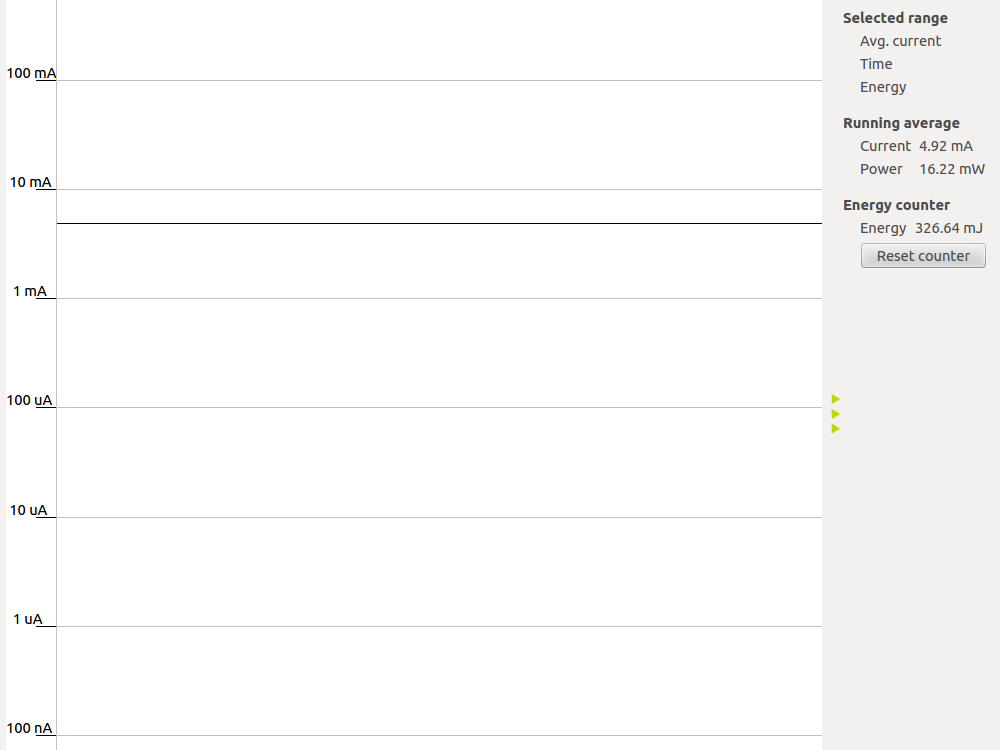
\includegraphics[width=\textwidth]{images/performance_with_polling.png}
 \caption{Energy consumpiton with polling}
\end{figure}

Our interrupt based program fared much better, averaging around 1.5$\mu$ A (fig), and expending about 83$\mu$ A when a button was held down. (fig)

In search of further improvement we powered down idle SRAM blocks to save more power, resulting in around 1$\mu$ A(fig), a pretty substantial improvement from the simple interrupt based program. With a button held down however the difference was negligible.(fig)
